\input{si.tex}



\section*{S1 Text : Extended Figures for Model Exploration}


\subsection*{Convergence}

% histograms


% and bimodal statistical distribution for cumulated points in the parameter space confirm the existence of superposed regimes : gaussian distribution gives stationary configurations, whereas inverse log-normal distribution are close to real data shape and correspond to non-stationary regime.
% -> not sure it is interesting to look at cumulated histograms.

% Figures :

%%%%%%%%%%%%%%%%%%%%
\begin{figure}
\centering
\includegraphics[width=\textwidth]{figuresraw/hist_moran}\\
\includegraphics[width=\textwidth]{figuresraw/hist_slope}
\caption{}
\label{}
\end{figure}
%%%%%%%%%%%%%%%%%%%%






\subsection*{Indicators Scatterplots}

% scatterplots - with real points


%%%%%%%%%%%%%
\begin{figure}
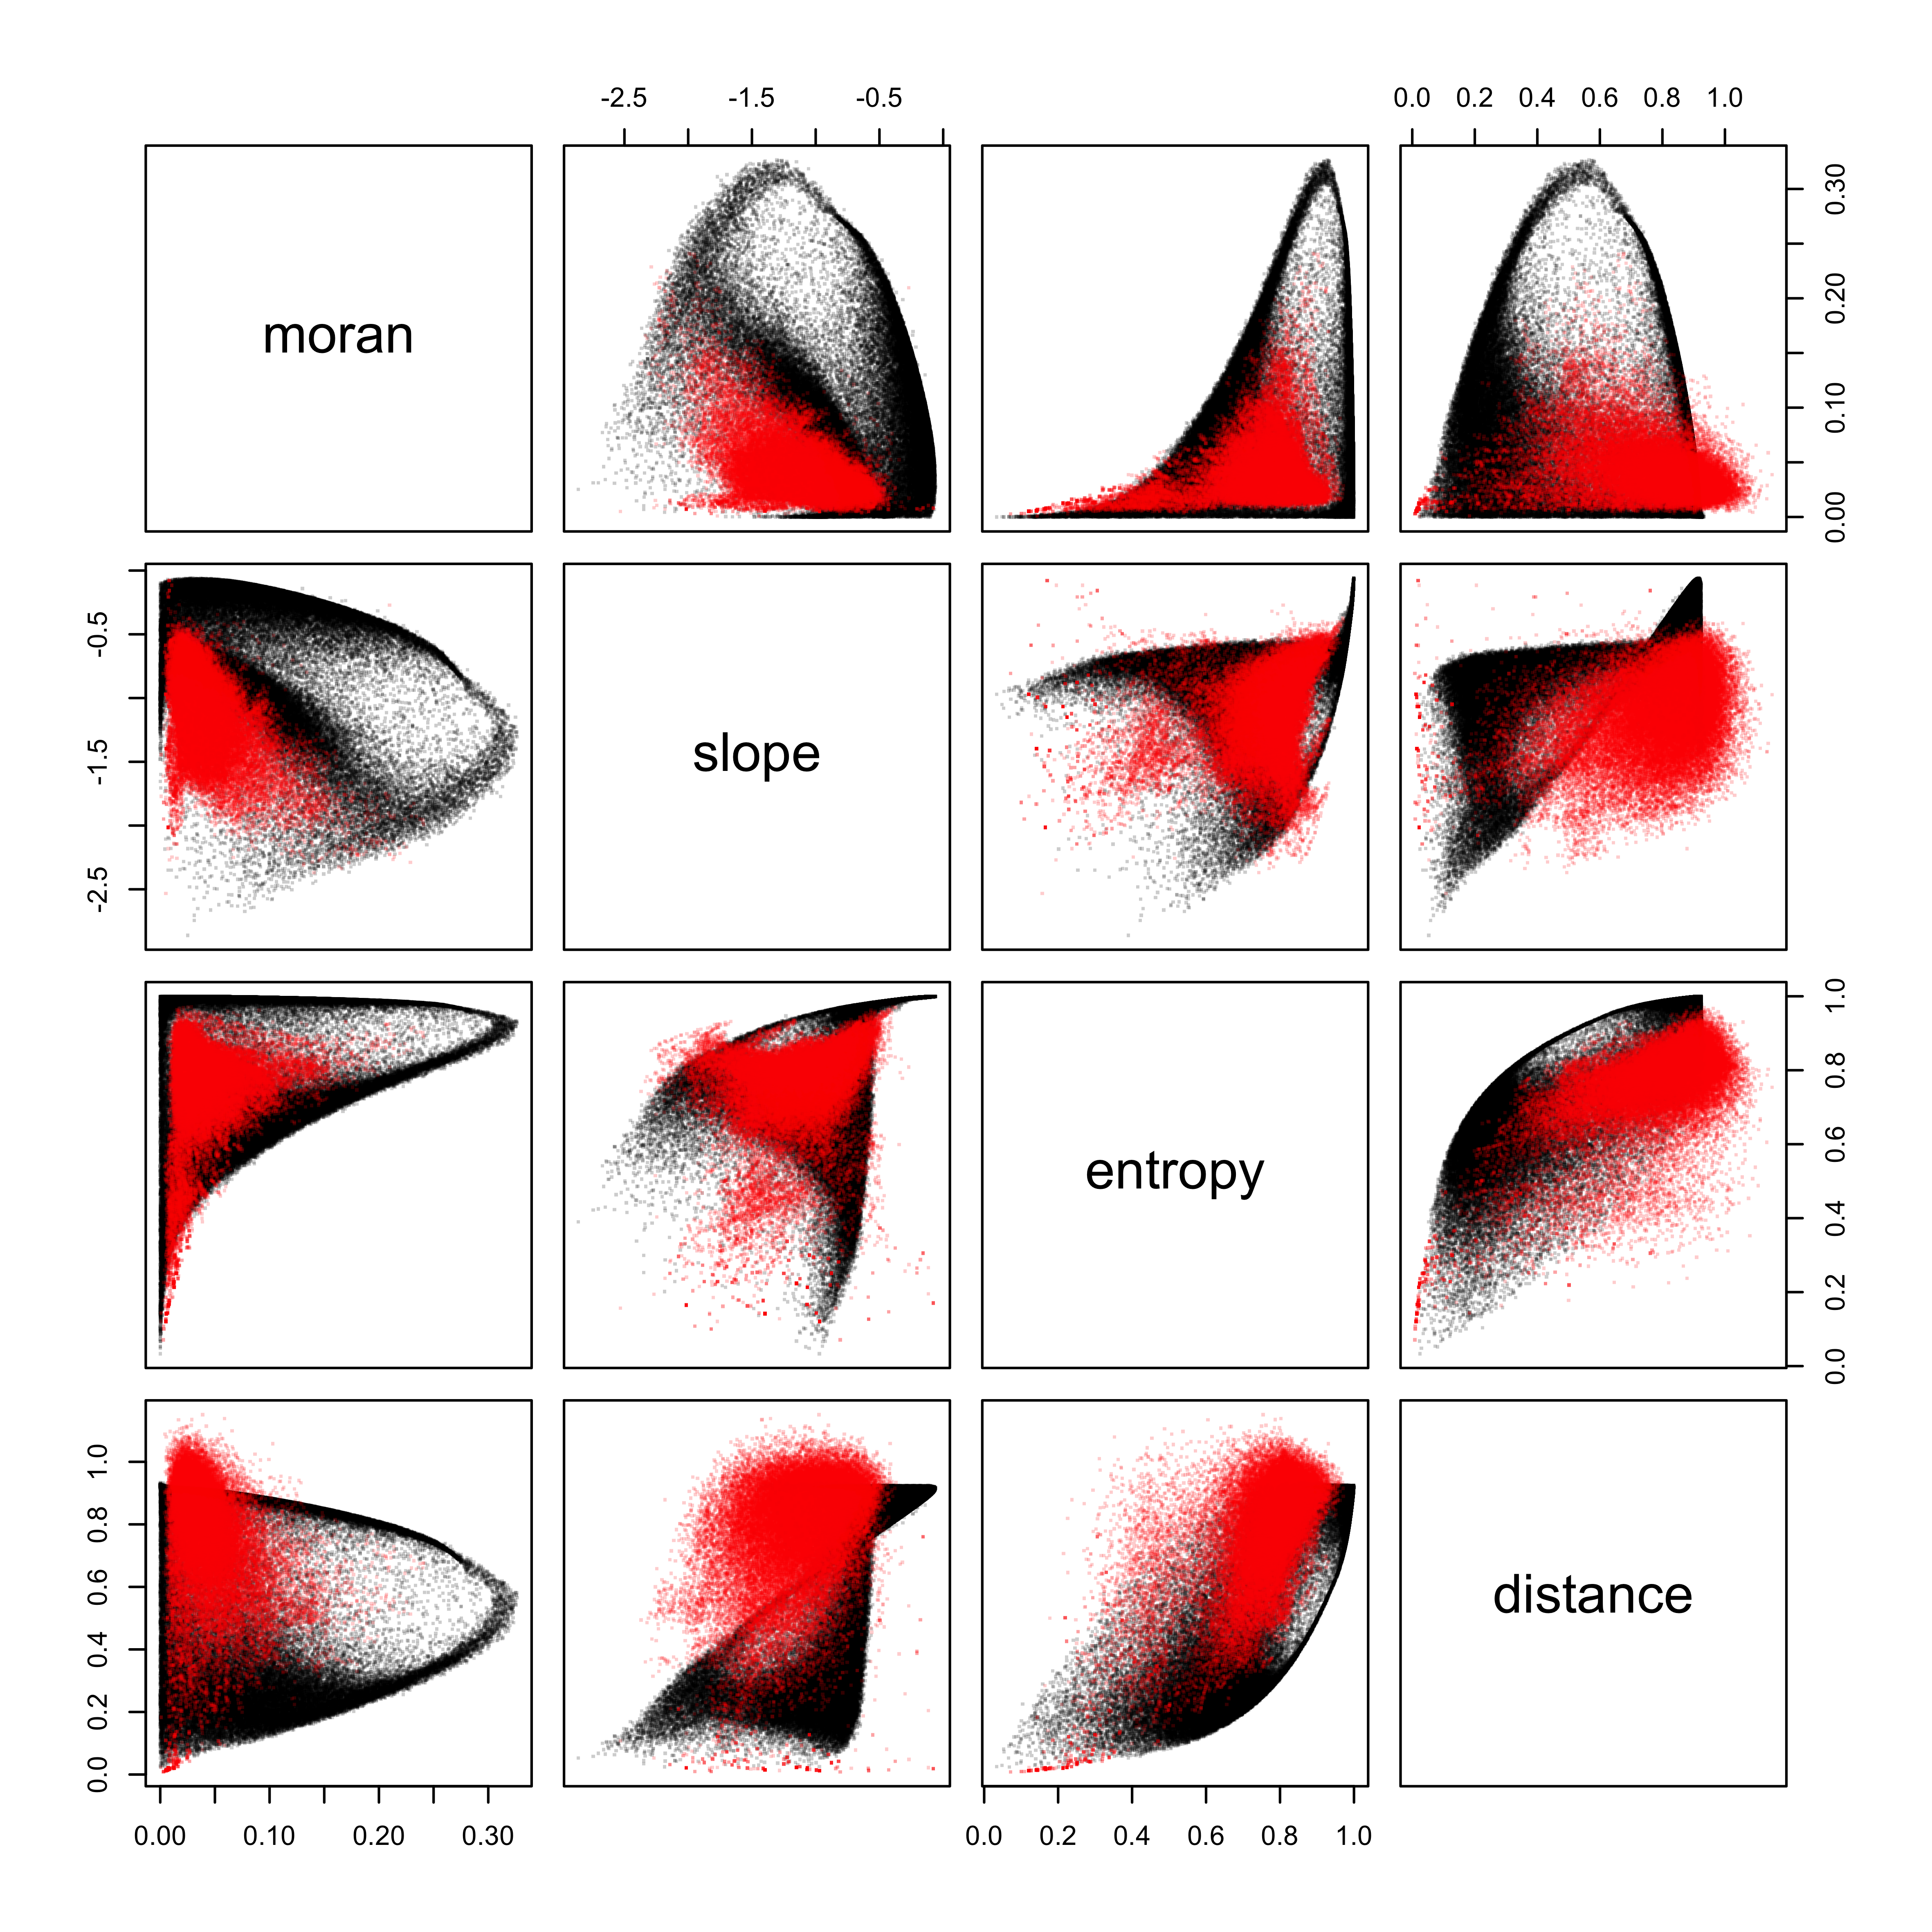
\includegraphics[width=\textwidth]{figuresraw/scatter}
\caption{Scatterplots of indicators distribution in an hypercube of the parameter space. Red points correspond to real data.}
\label{fig:densityscatter}
\end{figure}
%%%%%%%%%%%%%



\subsection*{Indicators Behavior}

% full plots behavior



%%%%%%%%%%%%%%%%%%%%
\begin{figure}
\centering
\includegraphics[width=\textwidth]{figuresraw/moran_alpha}
\includegraphics[width=\textwidth]{figuresraw/moran_beta}
\caption{Moran index as a function of $\alpha$ (Top) and $\beta$ (Bottom) for varying $\beta$ (resp. $\alpha$) given by color, and varying $n_d$ (row) and $N_G$}
\label{}
\end{figure}
%%%%%%%%%%%%%%%%%%%%

%%%%%%%%%%%%%%%%%%%%
\begin{figure}
\centering
\includegraphics[width=\textwidth]{figuresraw/slope_alpha}
\includegraphics[width=\textwidth]{figuresraw/slope_beta}
\caption{}
\label{}
\end{figure}
%%%%%%%%%%%%%%%%%%%%


%%%%%%%%%%%%%%%%%%%%
\begin{figure}
\centering
\includegraphics[width=\textwidth]{figuresraw/distance_alpha}
\includegraphics[width=\textwidth]{figuresraw/distance_beta}
\caption{}
\label{}
\end{figure}
%%%%%%%%%%%%%%%%%%%%

%%%%%%%%%%%%%%%%%%%%
\begin{figure}
\centering
\includegraphics[width=\textwidth]{figuresraw/entropy_alpha}
\includegraphics[width=\textwidth]{figuresraw/entropy_beta}
\caption{}
\label{}
\end{figure}
%%%%%%%%%%%%%%%%%%%%





\end{document}
